% !TEX program = lualatex
\documentclass[a4paper,10pt,oneside,openany]{ltjsreport}
\usepackage[margin=21mm,top=19mm,bottom=20mm]{geometry}
\usepackage[haranoaji]{luatexja-preset}
\usepackage{amsmath,amssymb,graphicx,booktabs,longtable,xcolor,float}
\usepackage[unicode,colorlinks=true,linkcolor=blue!45!black,urlcolor=blue!45!black]{hyperref}
\usepackage{caption}
\captionsetup{font=small,labelfont=bf}
\setcounter{tocdepth}{0}
\setlength{\parskip}{0.45em}
\setlength{\parindent}{1em}
\raggedbottom
\newcommand{\sourcefile}[1]{{\small\texttt{\detokenize{#1}}}}
\begin{document}


\title{\Huge 実験5\\[0.6em]\LARGE 粒子数とスピン偏極の同時変化\\[1em]\large 一次元HubbardモデルのUHF計算}

\author{保存結果の解析レポート}\date{2026年11月2日}\maketitle

\chapter*{概要}

$N_e=46,54$ と $\Delta N=0,4$ を組み合わせ、ドーピングと偏極を同時に比較する。$\Delta N=0$ の4ケースは未収束だが、4の4ケースは収束した。今回の条件では偏極が収束経路を変えたといえるが、一般に偏極させれば必ず収束が改善するという法則ではない。

対象は8ケース、保存図33枚である。収束は4ケース、未収束は4ケース。本書では生成物の種類ごとに章を設け、同じ条件のOBCとPBCを並べて読む。

\tableofcontents

\chapter{計算ログ：条件と最終結果}

\sourcefile{uhf_results.txt}

\section*{計算条件と量の定義}

$L=50$、$t=1$、温度 $T=0$、外部電場なし。全エネルギーと軌道エネルギーは $t$ を単位とする。
OBCは開放端、PBCはサイト50と1も接続する周期境界である。$N_e=N_\uparrow+N_\downarrow$、$\Delta N=N_\uparrow-N_\downarrow$ と定義する。
収束判定は混合前の密度残差 $r<10^{-10}$、最大反復回数は10000である。
表の「未」は未収束の最終再評価値であり、その桁数は精度保証ではない。

\begin{center}\small\setlength{\tabcolsep}{4pt}
\begin{longtable}{lrrrr}
\toprule
条件 & $N_e$ & $\Delta N$ & $U/t$ & mixing \\ \midrule
\endhead
Ne46\_dN00 & 46 & 0 & 4 & 0.25 \\
Ne46\_dN04 & 46 & 4 & 4 & 0.25 \\
Ne54\_dN00 & 54 & 0 & 4 & 0.25 \\
Ne54\_dN04 & 54 & 4 & 4 & 0.25 \\
\bottomrule\end{longtable}\end{center}

\section*{最終エネルギー}

$E=E_{\rm kin}+E_{\rm int}$、$E_{\rm int}=U\sum_i n_{i\uparrow}n_{i\downarrow}$。全エネルギーは占有軌道固有値の単純な総和ではなく、平均場の二重計数を除いた量である。

\begin{center}\small\setlength{\tabcolsep}{4pt}
\begin{longtable}{lrrrr}
\toprule
条件/境界 & 状態 & $E$ & $E_{\rm kin}$ & $E_{\rm int}$ \\ \midrule
\endhead
Ne46\_dN00/OBC & 未 & -26.320110741 & -46.133212224 & 19.813101482 \\
Ne46\_dN00/PBC & 未 & -26.763038523 & -46.912200597 & 20.149162074 \\
Ne46\_dN04/OBC & 収束 & -25.596394166 & -44.350493503 & 18.754099337 \\
Ne46\_dN04/PBC & 収束 & -26.039316343 & -45.134711903 & 19.095395560 \\
Ne54\_dN00/OBC & 未 & -10.320110741 & -46.133212224 & 35.813101482 \\
Ne54\_dN00/PBC & 未 & -10.763038939 & -46.912219496 & 36.149180557 \\
Ne54\_dN04/OBC & 収束 & -9.596394166 & -44.350493503 & 34.754099337 \\
Ne54\_dN04/PBC & 収束 & -10.039316343 & -45.134711903 & 35.095395560 \\
\bottomrule\end{longtable}\end{center}

$N_e=46,54$ と $\Delta N=0,4$ を組み合わせ、ドーピングと偏極を同時に比較する。$\Delta N=0$ の4ケースは未収束だが、4の4ケースは収束した。今回の条件では偏極が収束経路を変えたといえるが、一般に偏極させれば必ず収束が改善するという法則ではない。

\section*{原資料と再利用}

出典は \sourcefile{results_vault/experiment_05/} 内の各条件/OBC・PBCのログ、CSV、PNG。\\ 補助資料は \sourcefile{experiment_conditions.md} と \sourcefile{uhf.jl}。値は保存済みの結果から採り、SCFを再実行していない。

条件名は原資料のディレクトリ名である。dN00の両粒子数は実験3の再利用。

再利用データは独立した追加試行ではない。本書の解釈は保存された有限サイズ・UHF解の範囲に限る。

\chapter{密度CSV：電荷分布と二重占有}

\sourcefile{density_checkpoint.csv}

CSVの50サイトすべてから $q_i=n_{i\uparrow}+n_{i\downarrow}$、$m_i=n_{i\uparrow}-n_{i\downarrow}$、
$D=L^{-1}\sum_i n_{i\uparrow}n_{i\downarrow}$ を計算した。密度の各スピン成分は0以上1以下で、総和は指定した粒子数に一致することを確認した。未収束時のCSVは最後の混合密度を対角化して得た出力密度であり、固定点の密度とは限らない。

\begin{center}\small\setlength{\tabcolsep}{4pt}
\begin{longtable}{lrrrr}
\toprule
条件/境界 & 状態 & $\min q_i$ & $\max q_i$ & $D$ \\ \midrule
\endhead
Ne46\_dN00/OBC & 未 & 0.673299 & 0.999979 & 0.099066 \\
Ne46\_dN00/PBC & 未 & 0.695545 & 0.999832 & 0.100746 \\
Ne46\_dN04/OBC & 収束 & 0.588517 & 0.999972 & 0.093770 \\
Ne46\_dN04/PBC & 収束 & 0.589336 & 0.999525 & 0.095477 \\
Ne54\_dN00/OBC & 未 & 1.000021 & 1.326701 & 0.179066 \\
Ne54\_dN00/PBC & 未 & 1.000168 & 1.304226 & 0.180746 \\
Ne54\_dN04/OBC & 収束 & 1.000028 & 1.411483 & 0.173770 \\
Ne54\_dN04/PBC & 収束 & 1.000475 & 1.410664 & 0.175477 \\
\bottomrule\end{longtable}\end{center}

偏極4では、46のOBCで $q_i\simeq0.5885$ まで低下する局所的なホール領域があり、54のOBCでは対応して約1.4115まで増大する。PBCでもほぼ同じ密度範囲だが、変調の位置は異なる。平均密度0.92または1.08、平均磁化0.08を固定しても、局所密度は一様にはならない。

\chapter{SCFエネルギー：反復による変化}

\sourcefile{scf_energy.png}

収束した偏極4の組では、54と46の全エネルギー差はOBC・PBCとも16で、運動項は一致し、相互作用項だけが16ずれる。粒子・正孔対応と整合する。偏極0から4で最終記録のエネルギーは上がるが、偏極0は未収束なので、その差を収束状態間の偏極エネルギーとして確定してはならない。

各図の横軸は反復回数、縦軸は各反復で評価した全エネルギーである。図ごとに軸範囲が異なるため、見かけの傾きだけを比較しない。最終ログ値は反復終了後の再評価であり、履歴の最終点とわずかに異なる場合がある。

\begin{center}\small\setlength{\tabcolsep}{4pt}
\begin{longtable}{lrrr}
\toprule
条件/境界 & 初回 $E$ & 最終 $E$ & 最後の履歴の $|\Delta E|$ \\ \midrule
\endhead
Ne46\_dN00/OBC & -21.940669 & -26.320111 & $8.439\times10^{-9}$ \\
Ne46\_dN00/PBC & -22.628191 & -26.763039 & $1.436\times10^{-9}$ \\
Ne46\_dN04/OBC & -21.910261 & -25.596394 & $0$ \\
Ne46\_dN04/PBC & -22.559703 & -26.039316 & $0$ \\
Ne54\_dN00/OBC & -5.940669 & -10.320111 & $8.439\times10^{-9}$ \\
Ne54\_dN00/PBC & -6.628191 & -10.763039 & $8.100\times10^{-10}$ \\
Ne54\_dN04/OBC & -5.910261 & -9.596394 & $0$ \\
Ne54\_dN04/PBC & -6.559703 & -10.039316 & $0$ \\
\bottomrule\end{longtable}\end{center}

\begin{figure}[H]\centering

\begin{minipage}{0.49\linewidth}\centering

\textbf{OBC：未収束・暫定}\par

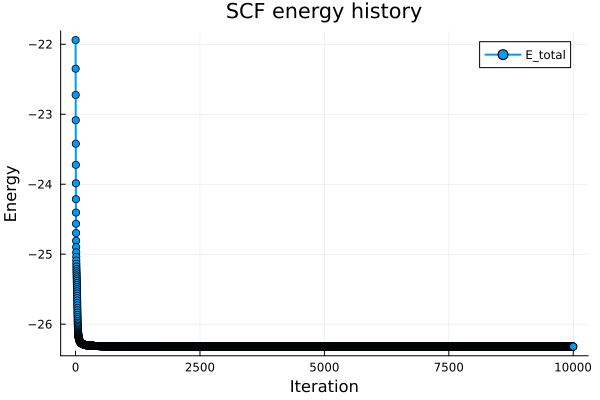
\includegraphics[width=\linewidth]{../../results_vault/experiment_05/Ne46_dN00/OBC/scf_energy.png}

\end{minipage}\hfill%
\begin{minipage}{0.49\linewidth}\centering

\textbf{PBC：未収束・暫定}\par

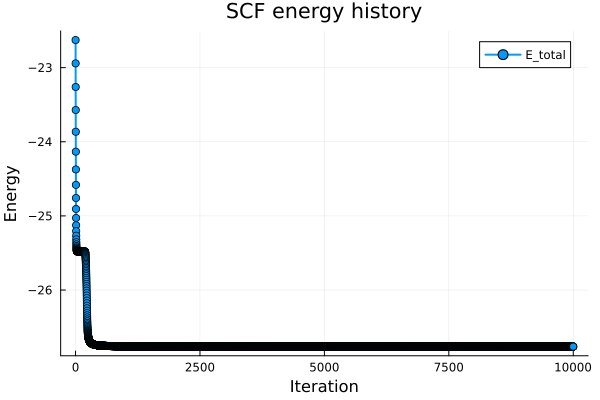
\includegraphics[width=\linewidth]{../../results_vault/experiment_05/Ne46_dN00/PBC/scf_energy.png}

\end{minipage}

\caption{Ne46\_dN00。SCFエネルギーの比較。左：OBC、右：PBC。}\end{figure}

\begin{figure}[H]\centering

\begin{minipage}{0.49\linewidth}\centering

\textbf{OBC：収束}\par

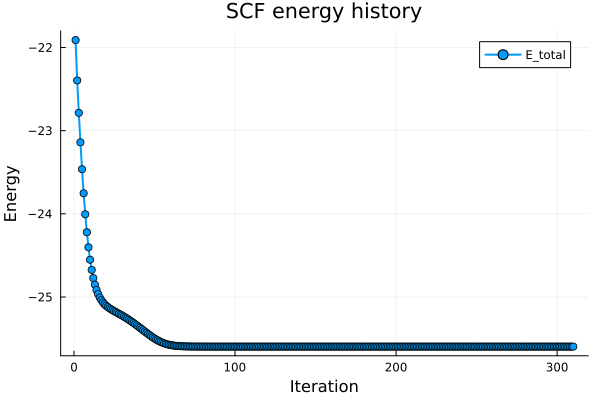
\includegraphics[width=\linewidth]{../../results_vault/experiment_05/Ne46_dN04/OBC/scf_energy.png}

\end{minipage}\hfill%
\begin{minipage}{0.49\linewidth}\centering

\textbf{PBC：収束}\par

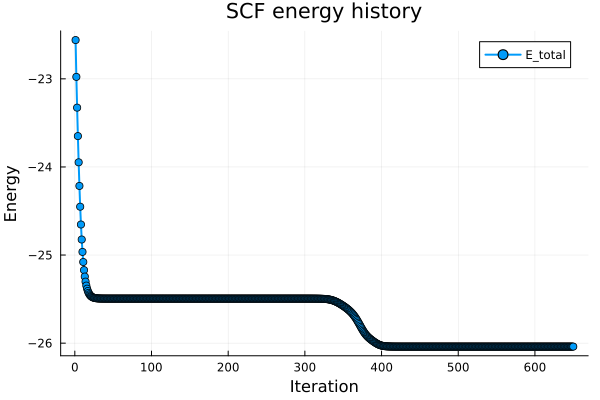
\includegraphics[width=\linewidth]{../../results_vault/experiment_05/Ne46_dN04/PBC/scf_energy.png}

\end{minipage}

\caption{Ne46\_dN04。SCFエネルギーの比較。左：OBC、右：PBC。}\end{figure}

\begin{figure}[H]\centering

\begin{minipage}{0.49\linewidth}\centering

\textbf{OBC：未収束・暫定}\par

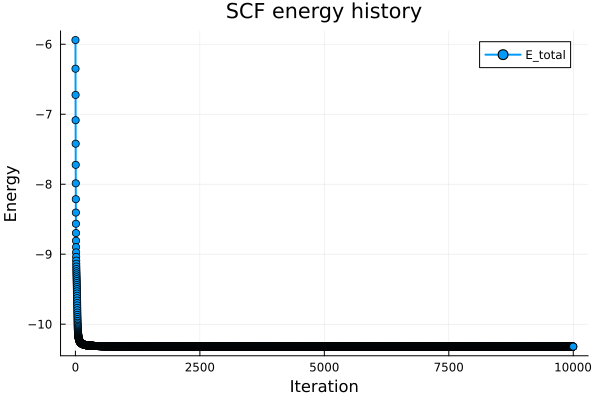
\includegraphics[width=\linewidth]{../../results_vault/experiment_05/Ne54_dN00/OBC/scf_energy.png}

\end{minipage}\hfill%
\begin{minipage}{0.49\linewidth}\centering

\textbf{PBC：未収束・暫定}\par

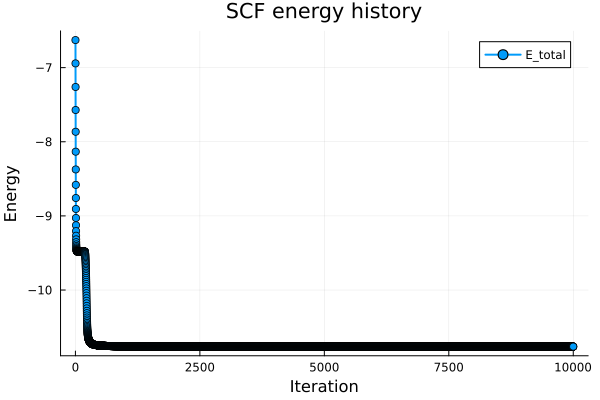
\includegraphics[width=\linewidth]{../../results_vault/experiment_05/Ne54_dN00/PBC/scf_energy.png}

\end{minipage}

\caption{Ne54\_dN00。SCFエネルギーの比較。左：OBC、右：PBC。}\end{figure}

\begin{figure}[H]\centering

\begin{minipage}{0.49\linewidth}\centering

\textbf{OBC：収束}\par

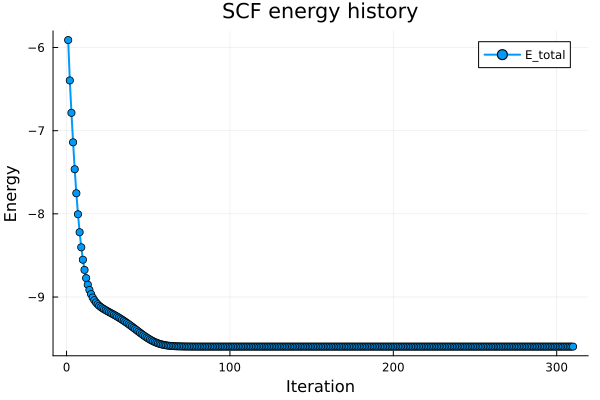
\includegraphics[width=\linewidth]{../../results_vault/experiment_05/Ne54_dN04/OBC/scf_energy.png}

\end{minipage}\hfill%
\begin{minipage}{0.49\linewidth}\centering

\textbf{PBC：収束}\par

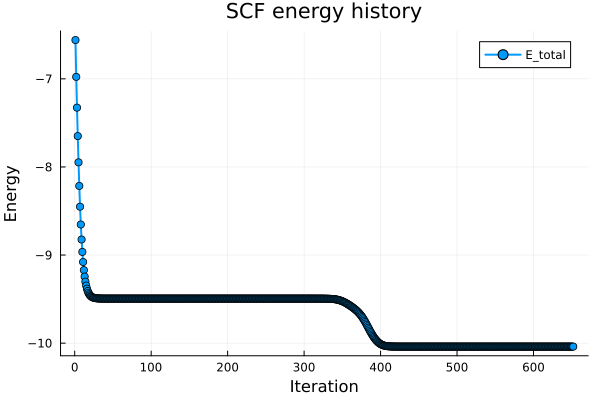
\includegraphics[width=\linewidth]{../../results_vault/experiment_05/Ne54_dN04/PBC/scf_energy.png}

\end{minipage}

\caption{Ne54\_dN04。SCFエネルギーの比較。左：OBC、右：PBC。}\end{figure}

\chapter{SCF残差：自己無撞着性}

\sourcefile{scf_residual.png}

偏極4のOBCは両粒子数で310反復、PBCは46で650反復、54で652反復を要した。PBCでは残差が一度小さくなった後に再増大し、エネルギーも後半にもう一段下がる。偏極0の平坦なエネルギー履歴と合わせ、エネルギーの停滞だけを終了条件にできないことが分かる。

残差は $r=\max_{i,\sigma}|F[n]_{i\sigma}-n_{i\sigma}|$。表は最終再評価値である。収束時には出力密度を採用してから再評価するため、履歴図の最後の残差とは同じとは限らない。

\begin{center}\small\setlength{\tabcolsep}{4pt}
\begin{longtable}{lrrr}
\toprule
条件/境界 & 状態 & 反復数 & 最終残差 \\ \midrule
\endhead
Ne46\_dN00/OBC & 未 & 10000 & $3.778\times10^{-5}$ \\
Ne46\_dN00/PBC & 未 & 10000 & $1.574\times10^{-5}$ \\
Ne46\_dN04/OBC & 収束 & 310 & $6.723\times10^{-11}$ \\
Ne46\_dN04/PBC & 収束 & 650 & $7.062\times10^{-11}$ \\
Ne54\_dN00/OBC & 未 & 10000 & $3.778\times10^{-5}$ \\
Ne54\_dN00/PBC & 未 & 10000 & $1.191\times10^{-5}$ \\
Ne54\_dN04/OBC & 収束 & 310 & $6.721\times10^{-11}$ \\
Ne54\_dN04/PBC & 収束 & 652 & $6.794\times10^{-11}$ \\
\bottomrule\end{longtable}\end{center}

\begin{figure}[H]\centering

\begin{minipage}{0.49\linewidth}\centering

\textbf{OBC：未収束・暫定}\par

\includegraphics[width=\linewidth]{../../results_vault/experiment_05/Ne46_dN00/OBC/scf_residual.png}

\end{minipage}\hfill%
\begin{minipage}{0.49\linewidth}\centering

\textbf{PBC：未収束・暫定}\par

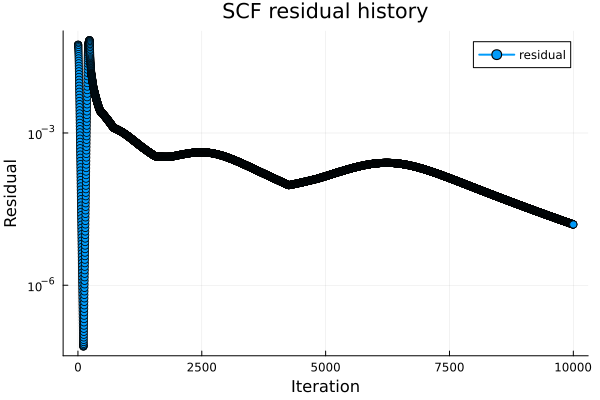
\includegraphics[width=\linewidth]{../../results_vault/experiment_05/Ne46_dN00/PBC/scf_residual.png}

\end{minipage}

\caption{Ne46\_dN00。SCF残差の比較。左：OBC、右：PBC。}\end{figure}

\begin{figure}[H]\centering

\begin{minipage}{0.49\linewidth}\centering

\textbf{OBC：収束}\par

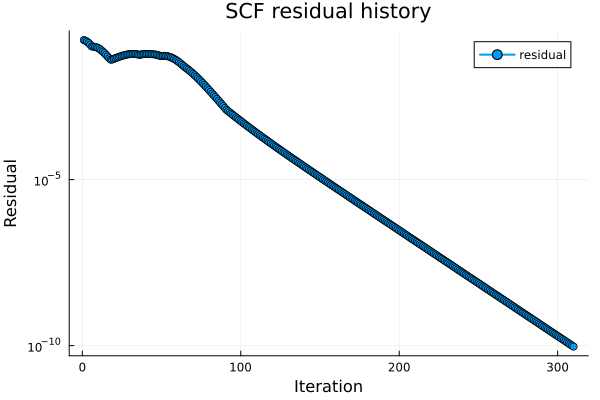
\includegraphics[width=\linewidth]{../../results_vault/experiment_05/Ne46_dN04/OBC/scf_residual.png}

\end{minipage}\hfill%
\begin{minipage}{0.49\linewidth}\centering

\textbf{PBC：収束}\par

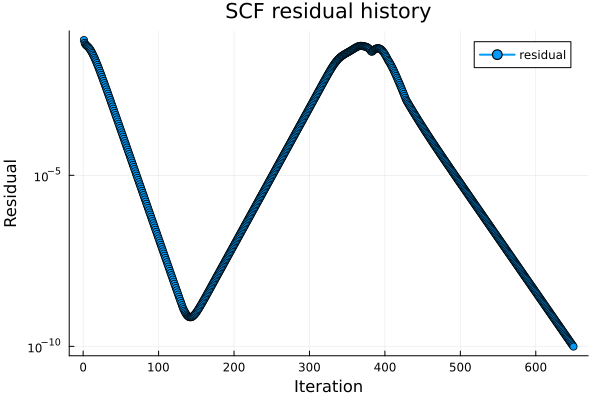
\includegraphics[width=\linewidth]{../../results_vault/experiment_05/Ne46_dN04/PBC/scf_residual.png}

\end{minipage}

\caption{Ne46\_dN04。SCF残差の比較。左：OBC、右：PBC。}\end{figure}

\begin{figure}[H]\centering

\begin{minipage}{0.49\linewidth}\centering

\textbf{OBC：未収束・暫定}\par

\includegraphics[width=\linewidth]{../../results_vault/experiment_05/Ne54_dN00/OBC/scf_residual.png}

\end{minipage}\hfill%
\begin{minipage}{0.49\linewidth}\centering

\textbf{PBC：未収束・暫定}\par

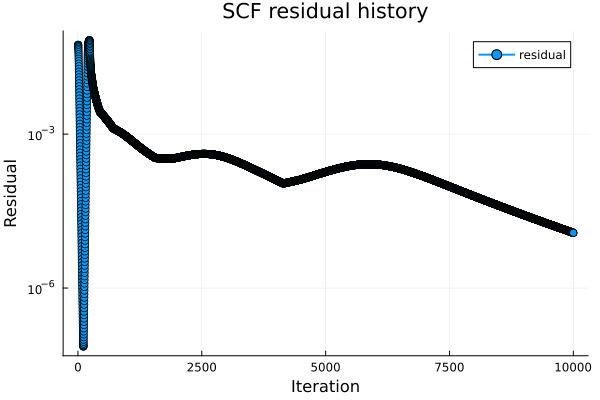
\includegraphics[width=\linewidth]{../../results_vault/experiment_05/Ne54_dN00/PBC/scf_residual.png}

\end{minipage}

\caption{Ne54\_dN00。SCF残差の比較。左：OBC、右：PBC。}\end{figure}

\begin{figure}[H]\centering

\begin{minipage}{0.49\linewidth}\centering

\textbf{OBC：収束}\par

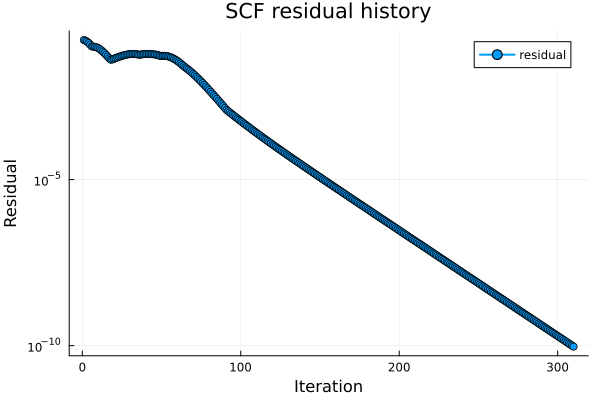
\includegraphics[width=\linewidth]{../../results_vault/experiment_05/Ne54_dN04/OBC/scf_residual.png}

\end{minipage}\hfill%
\begin{minipage}{0.49\linewidth}\centering

\textbf{PBC：収束}\par

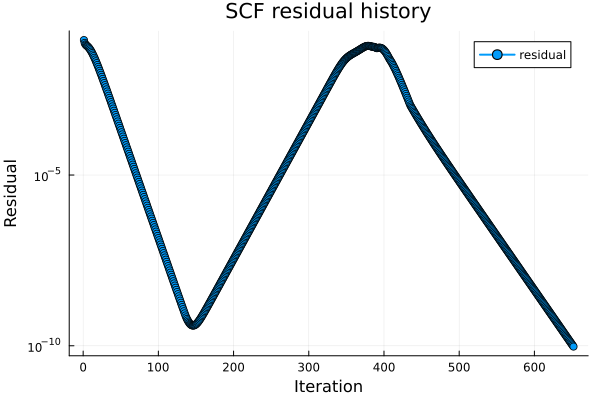
\includegraphics[width=\linewidth]{../../results_vault/experiment_05/Ne54_dN04/PBC/scf_residual.png}

\end{minipage}

\caption{Ne54\_dN04。SCF残差の比較。左：OBC、右：PBC。}\end{figure}

\chapter{軌道エネルギー：準位構造}

\sourcefile{final_orbital_energies.png}

偏極0では上下スピンの曲線は概ね重なるが、偏極4では中間準位の位置や段差が分かれる。46と54を比べると、電子数の増加に伴って平均場の準位全体の位置も変わる。横軸は各スピン内で独立にソートした番号であり、同じ番号が同じ空間軌道を表すとは限らない。

横軸はエネルギー昇順の軌道番号、縦軸は $h_\sigma=h_0+U\operatorname{diag}(n_{\bar\sigma})$ の固有値である。固有値の数値ファイルは保存されていないため、図からの解釈は定性的なものに留める。未収束例をCSVから再対角化すると保存図とは異なる平均場になる可能性があり、本書ではその置換を行わない。

\begin{figure}[H]\centering

\begin{minipage}{0.49\linewidth}\centering

\textbf{OBC：未収束・暫定}\par

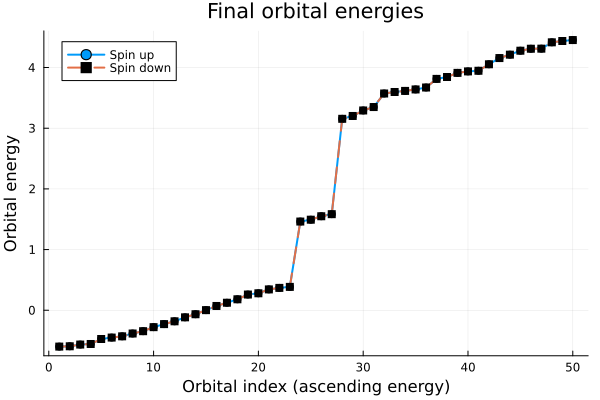
\includegraphics[width=\linewidth]{../../results_vault/experiment_05/Ne46_dN00/OBC/final_orbital_energies.png}

\end{minipage}\hfill%
\begin{minipage}{0.49\linewidth}\centering

\textbf{PBC：未収束・暫定}\par

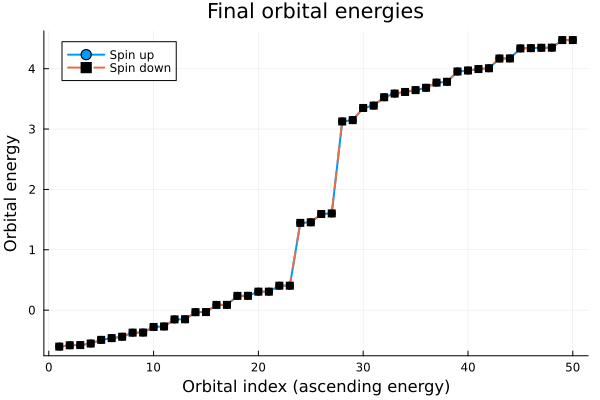
\includegraphics[width=\linewidth]{../../results_vault/experiment_05/Ne46_dN00/PBC/final_orbital_energies.png}

\end{minipage}

\caption{Ne46\_dN00。軌道エネルギーの比較。左：OBC、右：PBC。}\end{figure}

\begin{figure}[H]\centering

\begin{minipage}{0.49\linewidth}\centering

\textbf{OBC：収束}\par

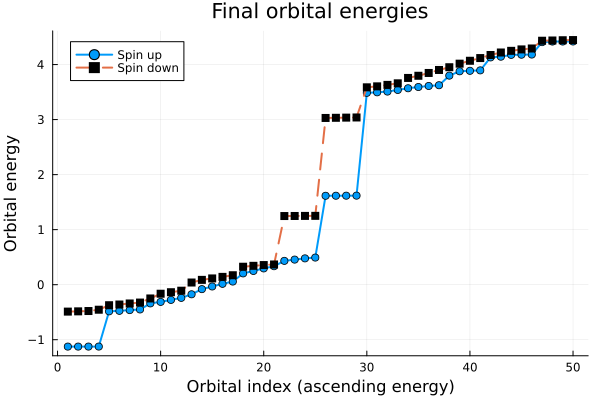
\includegraphics[width=\linewidth]{../../results_vault/experiment_05/Ne46_dN04/OBC/final_orbital_energies.png}

\end{minipage}\hfill%
\begin{minipage}{0.49\linewidth}\centering

\textbf{PBC：収束}\par

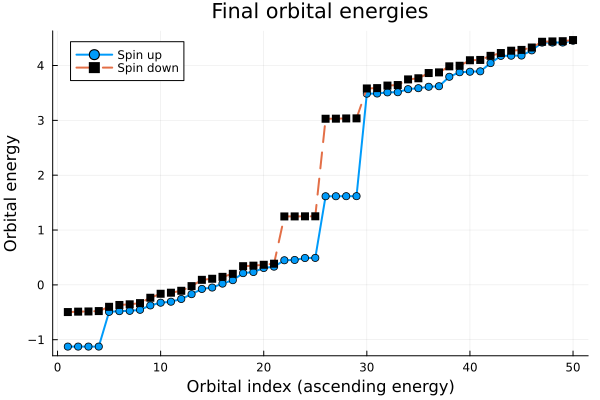
\includegraphics[width=\linewidth]{../../results_vault/experiment_05/Ne46_dN04/PBC/final_orbital_energies.png}

\end{minipage}

\caption{Ne46\_dN04。軌道エネルギーの比較。左：OBC、右：PBC。}\end{figure}

\begin{figure}[H]\centering

\begin{minipage}{0.49\linewidth}\centering

\textbf{OBC：未収束・暫定}\par

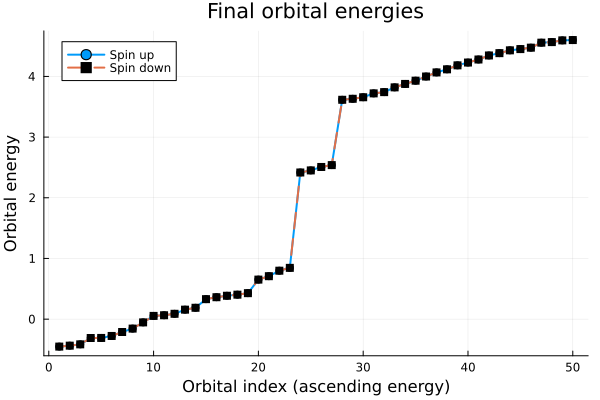
\includegraphics[width=\linewidth]{../../results_vault/experiment_05/Ne54_dN00/OBC/final_orbital_energies.png}

\end{minipage}\hfill%
\begin{minipage}{0.49\linewidth}\centering

\textbf{PBC：未収束・暫定}\par

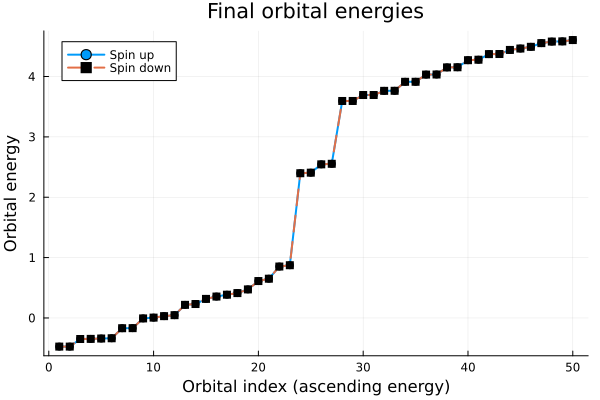
\includegraphics[width=\linewidth]{../../results_vault/experiment_05/Ne54_dN00/PBC/final_orbital_energies.png}

\end{minipage}

\caption{Ne54\_dN00。軌道エネルギーの比較。左：OBC、右：PBC。}\end{figure}

\begin{figure}[H]\centering

\begin{minipage}{0.49\linewidth}\centering

\textbf{OBC：収束}\par

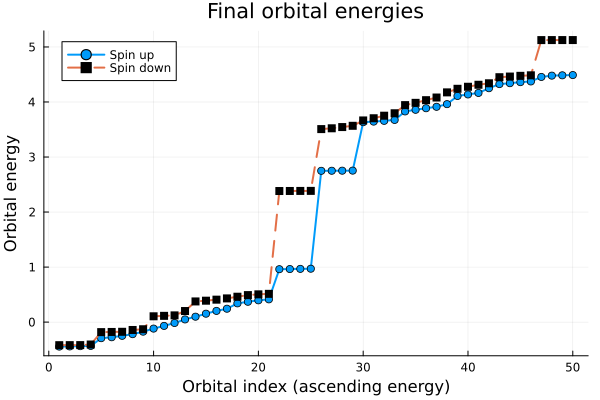
\includegraphics[width=\linewidth]{../../results_vault/experiment_05/Ne54_dN04/OBC/final_orbital_energies.png}

\end{minipage}\hfill%
\begin{minipage}{0.49\linewidth}\centering

\textbf{PBC：収束}\par

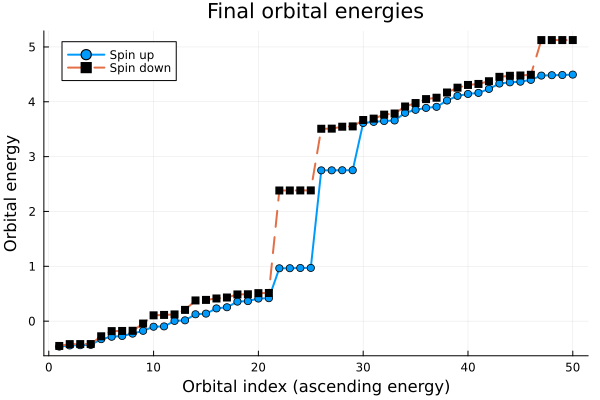
\includegraphics[width=\linewidth]{../../results_vault/experiment_05/Ne54_dN04/PBC/final_orbital_energies.png}

\end{minipage}

\caption{Ne54\_dN04。軌道エネルギーの比較。左：OBC、右：PBC。}\end{figure}

\chapter{局所磁化：空間構造}

\sourcefile{final_magnetization.png}

偏極4のOBCでは $\overline{|m|}=0.686891$、PBCでは0.682710で、46と54で一致する。OBCの交互磁化は0.617068であり、未収束の偏極0の0.244599より大きい。図でも偏極4では交互配列の保たれる領域が広いが、非偏極側が未収束であることを忘れてはならない。

$\overline{|m|}=L^{-1}\sum_i|m_i|$、$M_{\rm AF}=|L^{-1}\sum_i(-1)^im_i|$ と定義する。$m_i$ はスピン密度差であり、$\langle S_i^z\rangle=m_i/2$ に対応する。全磁化は $\sum_i m_i=\Delta N$ と粒子数制約で固定される。

\begin{center}\small\setlength{\tabcolsep}{4pt}
\begin{longtable}{lrrr}
\toprule
条件/境界 & 状態 & $\overline{|m|}$ & $M_{\rm AF}$ \\ \midrule
\endhead
Ne46\_dN00/OBC & 未 & 0.649298 & 0.244599 \\
Ne46\_dN00/PBC & 未 & 0.649121 & 0.205625 \\
Ne46\_dN04/OBC & 収束 & 0.686891 & 0.617068 \\
Ne46\_dN04/PBC & 収束 & 0.682710 & 0.612864 \\
Ne54\_dN00/OBC & 未 & 0.649298 & 0.244599 \\
Ne54\_dN00/PBC & 未 & 0.649116 & 0.205498 \\
Ne54\_dN04/OBC & 収束 & 0.686891 & 0.617068 \\
Ne54\_dN04/PBC & 収束 & 0.682710 & 0.612864 \\
\bottomrule\end{longtable}\end{center}

\begin{figure}[H]\centering

\begin{minipage}{0.49\linewidth}\centering

\textbf{OBC：未収束・暫定}\par

\includegraphics[width=\linewidth]{../../results_vault/experiment_05/Ne46_dN00/OBC/final_magnetization.png}

\end{minipage}\hfill%
\begin{minipage}{0.49\linewidth}\centering

\textbf{PBC：未収束・暫定}\par

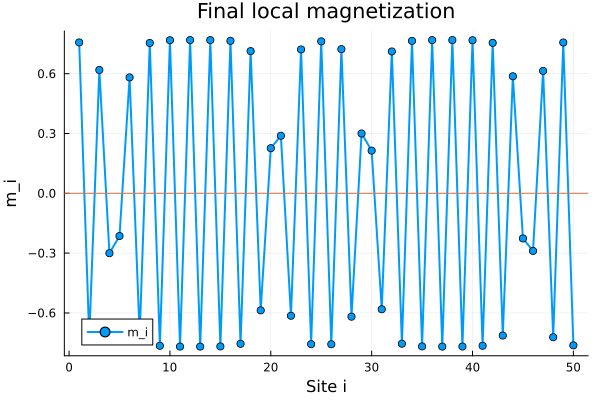
\includegraphics[width=\linewidth]{../../results_vault/experiment_05/Ne46_dN00/PBC/final_magnetization.png}

\end{minipage}

\caption{Ne46\_dN00。局所磁化の比較。左：OBC、右：PBC。}\end{figure}

\begin{figure}[H]\centering

\begin{minipage}{0.49\linewidth}\centering

\textbf{OBC：収束}\par

\includegraphics[width=\linewidth]{../../results_vault/experiment_05/Ne46_dN04/OBC/final_magnetization.png}

\end{minipage}\hfill%
\begin{minipage}{0.49\linewidth}\centering

\textbf{PBC：収束}\par

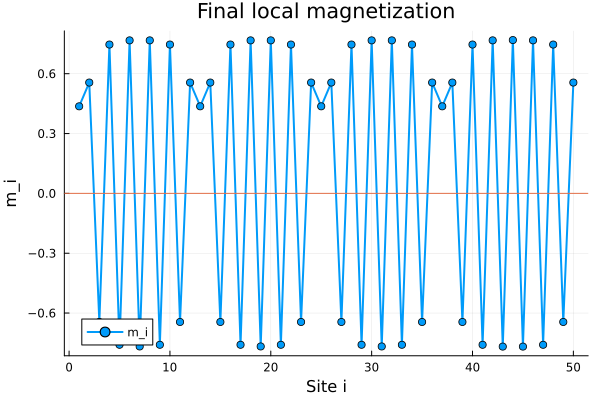
\includegraphics[width=\linewidth]{../../results_vault/experiment_05/Ne46_dN04/PBC/final_magnetization.png}

\end{minipage}

\caption{Ne46\_dN04。局所磁化の比較。左：OBC、右：PBC。}\end{figure}

\begin{figure}[H]\centering

\begin{minipage}{0.49\linewidth}\centering

\textbf{OBC：未収束・暫定}\par

\includegraphics[width=\linewidth]{../../results_vault/experiment_05/Ne54_dN00/OBC/final_magnetization.png}

\end{minipage}\hfill%
\begin{minipage}{0.49\linewidth}\centering

\textbf{PBC：未収束・暫定}\par

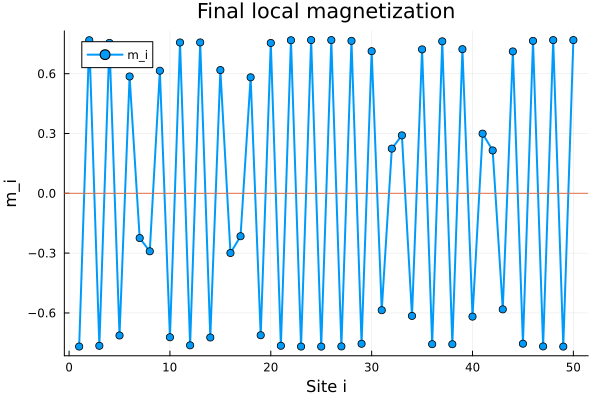
\includegraphics[width=\linewidth]{../../results_vault/experiment_05/Ne54_dN00/PBC/final_magnetization.png}

\end{minipage}

\caption{Ne54\_dN00。局所磁化の比較。左：OBC、右：PBC。}\end{figure}

\begin{figure}[H]\centering

\begin{minipage}{0.49\linewidth}\centering

\textbf{OBC：収束}\par

\includegraphics[width=\linewidth]{../../results_vault/experiment_05/Ne54_dN04/OBC/final_magnetization.png}

\end{minipage}\hfill%
\begin{minipage}{0.49\linewidth}\centering

\textbf{PBC：収束}\par

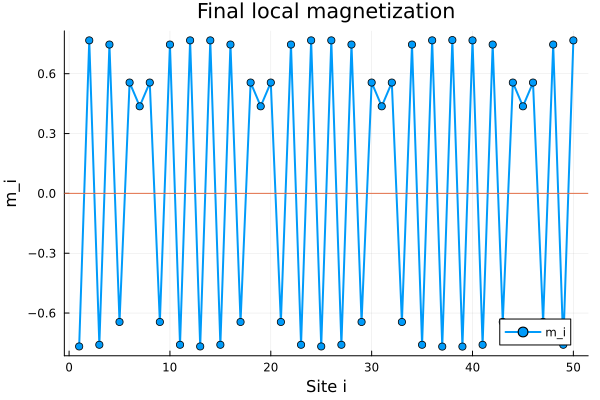
\includegraphics[width=\linewidth]{../../results_vault/experiment_05/Ne54_dN04/PBC/final_magnetization.png}

\end{minipage}

\caption{Ne54\_dN04。局所磁化の比較。左：OBC、右：PBC。}\end{figure}

\chapter{境界条件による全エネルギー差}

\sourcefile{boundary_energy_difference.png}

$\Delta E_{\rm boundary}=E_{\rm PBC}-E_{\rm OBC}$ と定義する。負ならPBC、正ならOBCの保存された解の方が低エネルギーである。両方が収束した組だけを表と図で数値比較し、それ以外をNCとする。

偏極4では両粒子数で $E_{\rm PBC}-E_{\rm OBC}=-0.442922176888$ と一致する。電子を加える側と取り去る側で、今回の対応する収束解の境界効果が一致したことを示す。偏極0の点はNCであり、両系列の差の大きさを比較するには非偏極側の収束が必要である。

\begin{center}\small\setlength{\tabcolsep}{4pt}
\begin{longtable}{lrr}
\toprule
条件 & $\Delta E_{\rm boundary}$ & $\Delta E_{\rm boundary}/L$ \\ \midrule
\endhead
Ne46\_dN00 & NC & NC \\
Ne46\_dN04 & -0.442922176888 & -0.008858443538 \\
Ne54\_dN00 & NC & NC \\
Ne54\_dN04 & -0.442922176888 & -0.008858443538 \\
\bottomrule\end{longtable}\end{center}

\begin{figure}[H]\centering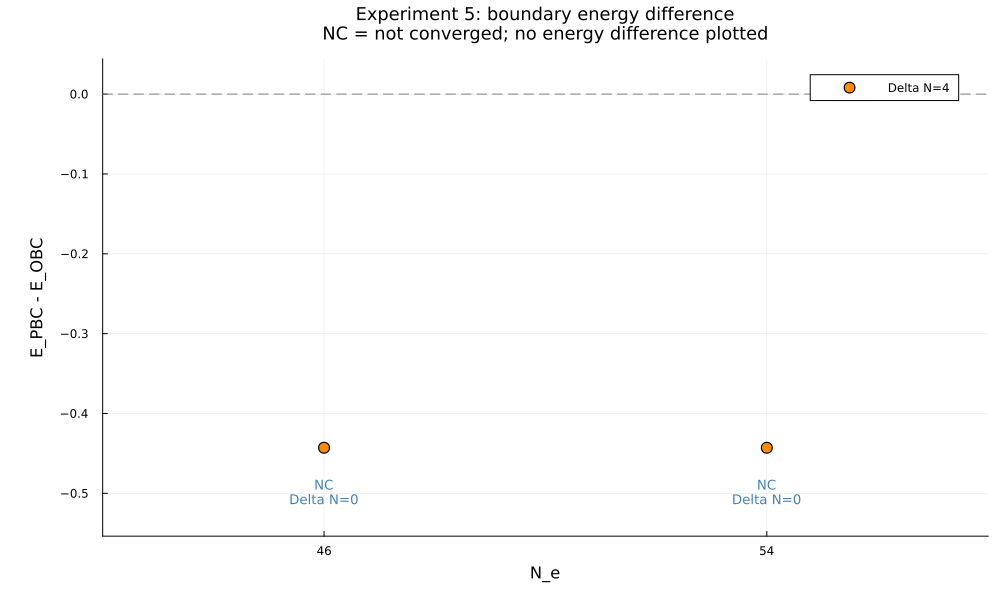
\includegraphics[width=0.9\linewidth]{../../results_vault/experiment_05/boundary_energy_difference.png}\caption{保存済みの境界エネルギー差。NCは未収束の組を示し、差が0であることを意味しない。}\end{figure}

\section*{結論と残された確認}

$N_e=46,54$ と $\Delta N=0,4$ を組み合わせ、ドーピングと偏極を同時に比較する。$\Delta N=0$ の4ケースは未収束だが、4の4ケースは収束した。今回の条件では偏極が収束経路を変えたといえるが、一般に偏極させれば必ず収束が改善するという法則ではない。

未収束ケースについては残差を満たす解を得た上で、複数の初期密度から同じ状態に到達するかを確認する必要がある。

サイズは50に固定しているため、境界効果と有限サイズ効果の切り分けには別サイズの結果が必要である。

\end{document}